\newpage
\subsection{}

$
\begin{bmatrix}
(\chi \land \bigcirc^{2} \psi) \rightarrow \bigcirc^{2} (\tau \textbf{W} \omega) \\
\mu \rightarrow \bigcirc^{5} \omega
\end{bmatrix}
$

\subsubsection{Description}
\begin{itemize}
    \item The first statement reads as if at time i, $\chi$ is true and in the next 2 states, $\psi$ is true, then from (i+2), $\tau$ is true unless $\omega$ is true (however, there's no guarantee that $\omega$ will be true in the future).
    \item The second statement reads as if at time i, $\mu$ is true then at (i+5), $\omega$ must be true
    \item[] $\rightarrow$ Combining the 2 statements logically, we have: if $\chi$ and $\mu$ are true at time i, and $\psi$ is true at time i+2, then $\tau$ is true at (i+2), (i+3), (i+4) and $\omega$ is true at (i+5)
\end{itemize}

\subsubsection{Visualization}

% Start section
\begin{figure}[h!]
	\centering 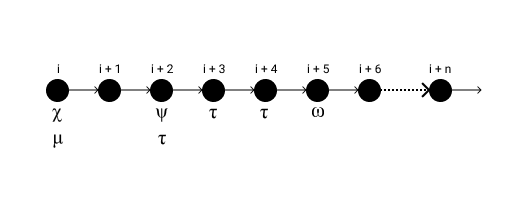
\includegraphics[width=1\textwidth]{Problem2-8}
\end{figure}
